\documentclass[11pt]{article}
\usepackage{acl}
\usepackage{times}
\usepackage{latexsym}
\usepackage{amsmath,amssymb}
\usepackage{graphicx}
\usepackage{booktabs}
\usepackage{url}

\setcitestyle{numbers}   % 新增：强制数字引用，解决 natbib 报错

\title{Giant Components under Random Failures: A Mini Review from Single-Layer to Multilayer Networks}

\author{Chenhua Zhu \\
  QHNU \\
  \texttt{zhu.chenhua@qq.com} \\
  \texttt{https://github.com/ZhuChenHua/study-multilayer-networks}}

\date{}

\begin{document}
\maketitle

\begin{abstract}
  Understanding how networks remain connected under random failures is a central problem in network science. This mini review introduces the basic concepts of connected components, the largest connected component, and the giant component under random attacks. We first review the generating-function formalism for single-layer networks and derive the classic Erd\H{o}s--R\'enyi result. We then move to multilayer interdependent networks, where the mutually connected giant component (MCGC) emerges through a discontinuous phase transition. A small numerical experiment compares single-layer and two-layer ER networks, and the complete simulation code is available online.
\end{abstract}

\section{Introduction}
Many real-world systems---power grids, the Internet, social platforms, and transportation networks---can be modeled as networks. A fundamental question is how robust these networks are when a fraction of nodes is randomly removed or fails. This process is often studied through percolation theory, where one asks whether a giant connected component still exists after random damage.

In single-layer networks, the answer is relatively well understood. For random graphs and configuration models, generating functions give the size of the giant component and the percolation threshold. In multilayer networks, however, the picture changes dramatically. When nodes in different layers depend on each other, a failure in one layer can trigger cascading failures in other layers, leading to a discontinuous collapse of the mutually connected giant component.

This mini review is intended for students who are new to network percolation. We focus on the core definitions, the main formulas, and one small numerical experiment. The full simulation code is available at \url{https://github.com/ZhuChenHua/study-multilayer-networks}.

\section{Definitions and Random Failure Model}
Let $G=(V,E)$ be an undirected graph with $N=|V|$ nodes. A \emph{connected component} is a maximal subset $C\subseteq V$ such that the induced subgraph $G[C]$ is connected. The \emph{largest connected component} is
\begin{equation}
  C_{\max} = \arg\max_{C\in \mathcal{C}(G)} |C|,
\end{equation}
where $\mathcal{C}(G)$ is the set of all connected components. If $|C_{\max}|$ scales linearly with $N$, it is called the \emph{giant component}.

In the random failure model, each node is removed independently with probability $q$. Equivalently, each node remains with probability $p=1-q$. After removal, we consider the induced subgraph on the remaining nodes. The quantity of interest is the ratio
\begin{equation}
  R(q) = \frac{|C_{\max}(G_q)|}{N},
\end{equation}
where $G_q$ is the remaining graph. We also use $S(q)$ to denote the giant component size relative to the original network.

\section{Single-Layer Percolation}
\subsection{Generating functions}
For a configuration-model network with degree distribution $P(k)$, define the generating functions
\begin{equation}
  G_0(x)=\sum_k P(k)x^k,\qquad
  G_1(x)=\sum_k \frac{kP(k)}{\langle k\rangle}x^{k-1}.
\end{equation}
After random removal with probability $q$, let $u$ be the probability that a randomly chosen edge does not lead to the giant component. Then
\begin{equation}
  u = q + p G_1(u),
\end{equation}
and the giant component fraction is
\begin{equation}
  S = p[1-G_0(u)].
\end{equation}
The percolation threshold is determined by the first non-trivial solution of these equations.

\subsection{Erd\H{o}s--R\'enyi networks}
For an Erd\H{o}s--R\'enyi (ER) network with average degree $c$, we have
\begin{equation}
  G_0(x)=G_1(x)=e^{-c(1-x)}.
\end{equation}
Thus the giant component fraction satisfies
\begin{equation}
  S = p(1-e^{-cS}) = (1-q)(1-e^{-cS}).
\end{equation}
The critical point is
\begin{equation}
  p_c = \frac{1}{c},\qquad q_c = 1-\frac{1}{c}.
\end{equation}
For $q<q_c$, a giant component exists; for $q>q_c$, it disappears.

\section{Multilayer Interdependent Networks}
In a multiplex or interdependent network, each node has a replica in every layer. A node is active only if it belongs to the giant component in all layers. The largest set of such nodes is called the \emph{mutually connected giant component} (MCGC).

Consider $M$ layers, each an ER network with average degree $c$. After random removal with probability $q$, the MCGC fraction $S$ satisfies
\begin{equation}
  S = p(1-e^{-cS})^M = (1-q)(1-e^{-cS})^M.
\end{equation}
For $M=1$, this reduces to the single-layer ER result. For $M\ge 2$, the transition becomes discontinuous. The critical point is found by solving
\begin{equation}
  g_y(x)=x-y(1-e^{-x})^M=0,
  \qquad
  g_y'(x)=0,
\end{equation}
where $y=cp=c(1-q)$. For $M=2$, one obtains $y_c\approx 2.45541$, so
\begin{equation}
  q_c = 1-\frac{y_c}{c}.
\end{equation}
This shows that interdependencies make the network more fragile: the transition is abrupt, and cascading failures can destroy the entire system.

\section{Numerical Experiments}
We perform a small simulation to illustrate the theory. We generate ER networks with $N=10{,}000$ nodes and average degree $c=4$. For the multilayer case, we generate two independent ER layers and couple each node with its replica in the other layer. We remove a fraction $q$ of nodes randomly, compute the largest connected component for the single-layer case and the MCGC for the two-layer case, and average over 20 independent runs.

Figure~\ref{fig:result} shows the results. The single-layer network exhibits a continuous transition near $q_c=0.75$, while the two-layer interdependent network collapses discontinuously at a smaller value of $q$. The simulation points agree well with the theoretical curves obtained from Eqs.~(6) and (9).

\begin{figure}[t]
  \centering
  % 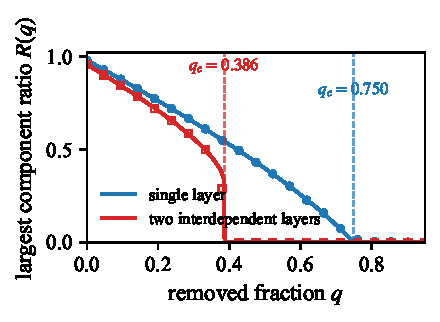
\includegraphics[width=\columnwidth]{figures/giant_component.pdf}
  \caption{Largest connected component ratio $R(q)$ under random failures. Markers: simulation; lines: theory. Single-layer ER network (blue) and two-layer interdependent ER network (red). The multilayer transition is discontinuous and occurs earlier.}
  \label{fig:result}
\end{figure}

\section{Conclusion and Code}
This mini review summarized the basics of random failures and giant components in single-layer and multilayer networks. The single-layer case is described by generating functions and the ER formula $S=(1-q)(1-e^{-cS})$. In multilayer interdependent networks, the MCGC follows $S=(1-q)(1-e^{-cS})^M$, and the transition becomes discontinuous for $M\ge 2$. A small numerical experiment confirmed these predictions.

The complete simulation code, including network generation, random removal, BFS-based component detection, and plotting scripts, is available at
\begin{center}
  \url{https://github.com/ZhuChenHua/study-multilayer-networks}.
\end{center}
Students are encouraged to modify the parameters $N$, $c$, $q$, and $M$ to explore different regimes.

\begin{thebibliography}{99}
  \bibitem{erdos1960}
  P. Erd\H{o}s and A. R\'enyi.
  \newblock On the evolution of random graphs.
  \newblock \emph{Publications of the Mathematical Institute of the Hungarian Academy of Sciences}, 5:17--61, 1960.

  \bibitem{molloy1995}
  M. Molloy and B. Reed.
  \newblock A critical point for random graphs with a given degree sequence.
  \newblock \emph{Random Structures \& Algorithms}, 6(2-3):161--180, 1995.

  \bibitem{callaway2000}
  D. S. Callaway, M. E. J. Newman, S. H. Strogatz, and D. J. Watts.
  \newblock Network robustness and fragility: Percolation on random graphs.
  \newblock \emph{Physical Review Letters}, 85(25):5468--5471, 2000.

  \bibitem{cohen2000}
  R. Cohen, K. Erez, D. ben-Avraham, and S. Havlin.
  \newblock Resilience of the Internet to random breakdowns.
  \newblock \emph{Physical Review Letters}, 85(21):4626--4628, 2000.

  \bibitem{buldyrev2010}
  S. V. Buldyrev, R. Parshani, G. Paul, H. E. Stanley, and S. Havlin.
  \newblock Catastrophic cascade of failures in interdependent networks.
  \newblock \emph{Nature}, 464(7291):1025--1028, 2010.

  \bibitem{parshani2010}
  R. Parshani, S. V. Buldyrev, and S. Havlin.
  \newblock Interdependent networks: Reducing the coupling strength leads to a change from a first to second order percolation transition.
  \newblock \emph{Physical Review Letters}, 105(4):048701, 2010.

  \bibitem{gao2011}
  J. Gao, S. V. Buldyrev, S. Havlin, and H. E. Stanley.
  \newblock Robustness of a network of networks.
  \newblock \emph{Physical Review Letters}, 107(19):195701, 2011.

  \bibitem{boccaletti2014}
  S. Boccaletti, G. Bianconi, R. Criado, C. I. del Genio, J. G\'omez-Garde\~nes, M. Romance, I. Sendi\~na-Nadal, Z. Wang, and M. Zanin.
  \newblock The structure and dynamics of multilayer networks.
  \newblock \emph{Physics Reports}, 544(1):1--122, 2014.

  \bibitem{kivela2014}
  M. Kivel\"a, A. Arenas, M. Barthelemy, J. P. Gleeson, Y. Moreno, and M. A. Porter.
  \newblock Multilayer networks.
  \newblock \emph{Journal of Complex Networks}, 2(3):203--271, 2014.

  \bibitem{newman2010}
  M. E. J. Newman.
  \newblock \emph{Networks: An Introduction}.
  \newblock Oxford University Press, 2010.
\end{thebibliography}

\end{document}